\chapter{Produção de Conteúdo}
\label{chap:producaoConteudo}

O Noosfero foi pensado inicialmente como sendo uma plataforma para Redes Sociais, e por conta disso, tem uma estrutura de conteúdo diferenciada comparada a outros CMS como Joomla.

No Noosfero todo conteúdo deve estar contido dentro de uma comunidade, por isso aprenderemos primeiro a seção \emph{\hyperref[sec:criarComunidade]{criação de comunidade}} e a partir disso apresentaremos a seção \emph{\hyperref[sec:criarConteudo]{criação de artigo, pasta ou blog}}.

\section{Criação de comunidade}
\label{sec:criarComunidade}

A comunidade é a base para qualquer conteúdo publicado na plataforma Noosfero, pois qualquer conteúdo deve estar contido em uma comunidade.

Para a criação de uma comunidade deve-se clicar em \emph{\color{red}Painel de Controle} localizado no rodapé da página.

\begin{figure}[H]
  \centering
    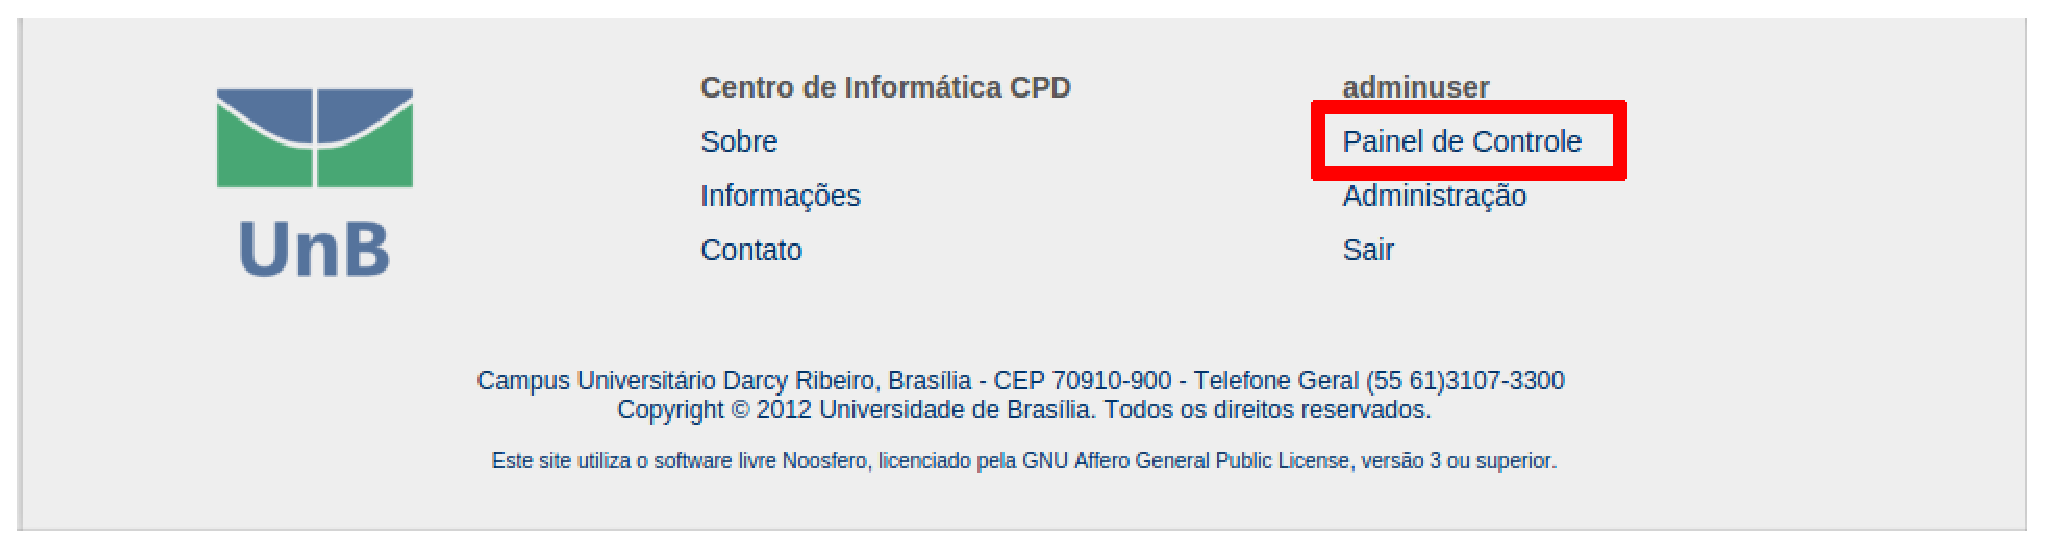
\includegraphics[keepaspectratio=true,scale=0.49]{figuras/linkPainelControle.eps}    
  \caption{Link para o Painel de Controle.}
  \label{fig:linkPainelControle}
\end{figure}

\newpage
Dentro do painel de controle, clique em \emph{\color{red}Gerenciar meus grupos}.

\begin{figure}[H]
  \centering
    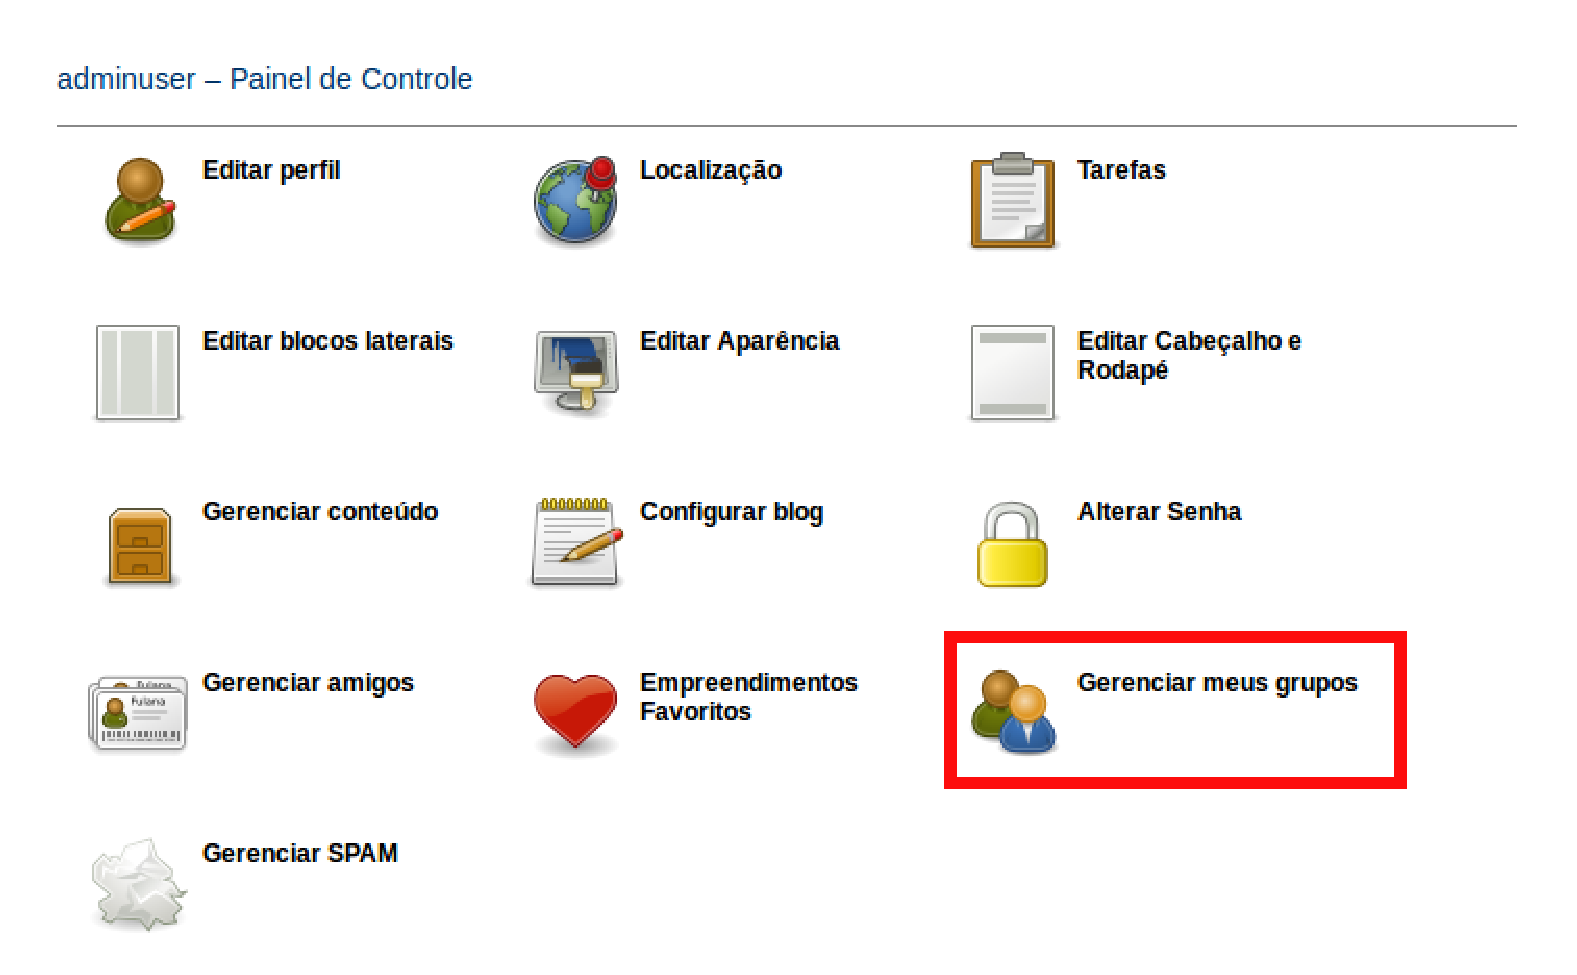
\includegraphics[keepaspectratio=true,scale=0.49]{figuras/painelDeControle.eps}
  \caption{Gerenciar grupos no painel de controle.}
  \label{fig:GerGrupPainelControle}
\end{figure}

E finalmente em \emph{\color{red}Criar nova comunidade}.

\begin{figure}[H]
  \centering
    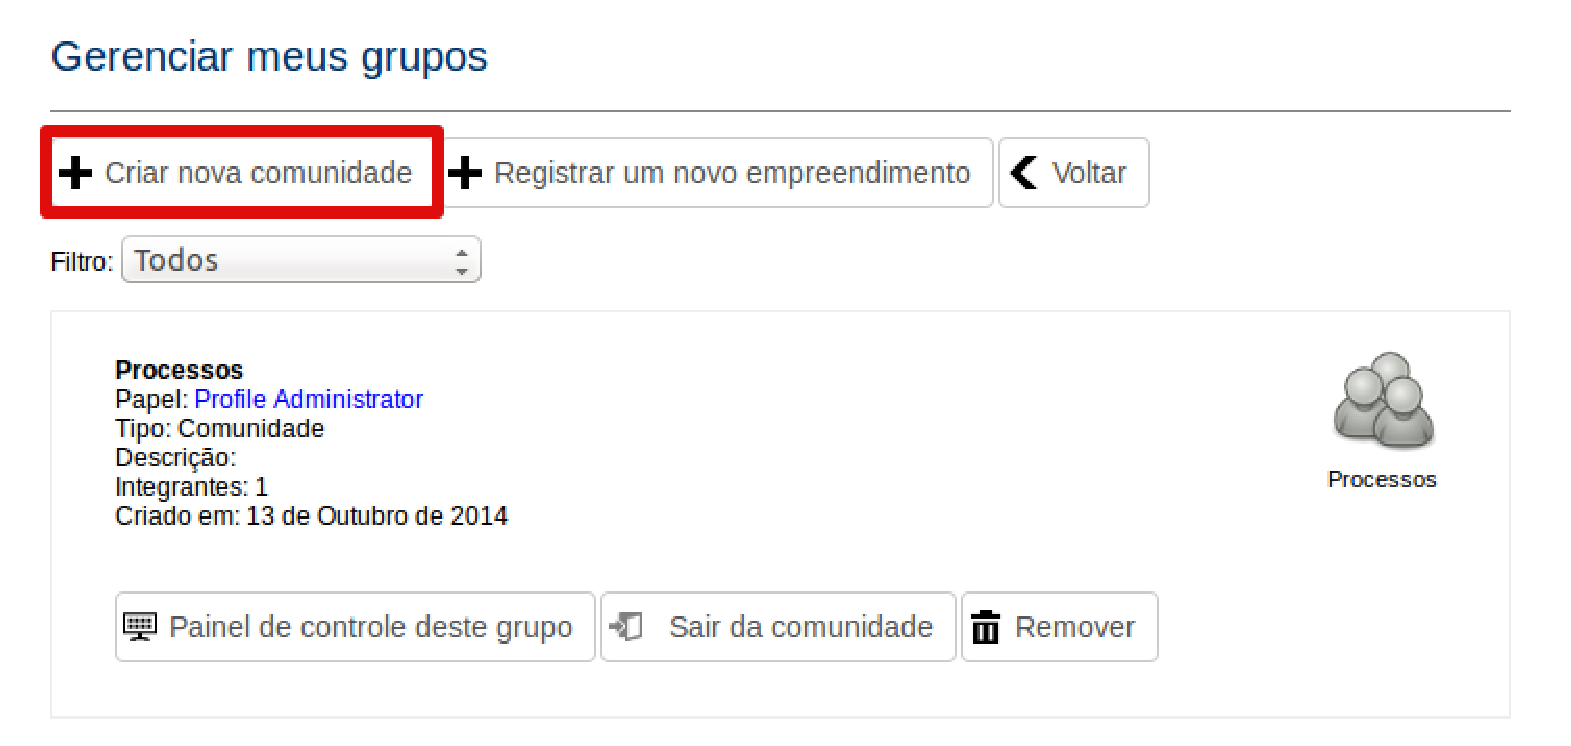
\includegraphics[keepaspectratio=true,scale=0.49]{figuras/gerenciarGrupos.eps}
  \caption{Botão de acesso para criar comunidade.}
  \label{fig:botaoAcesso}
\end{figure}

\newpage
Agora basta dar um nome para a comunidade e clicar no botão \emph{\color{red}Criar}.

\begin{figure}[H]
  \centering
    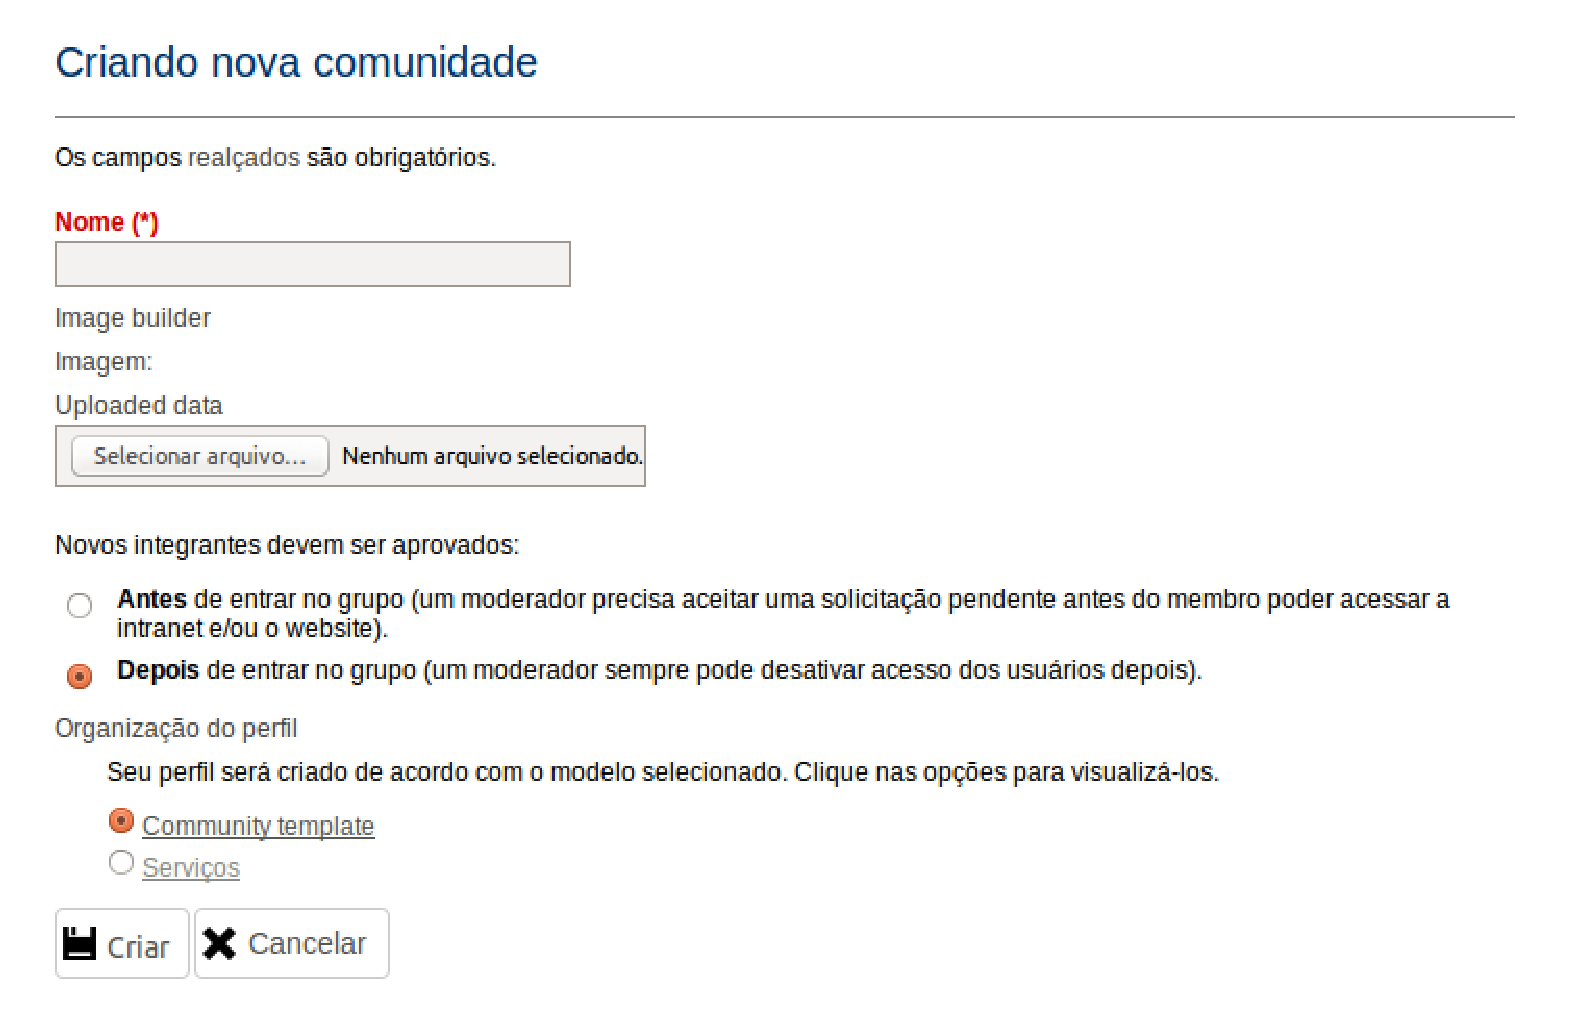
\includegraphics[keepaspectratio=true,scale=0.49]{figuras/criandoComunidade.eps}
  \caption{Formulário de criação da comunidade.}
  \label{fig:criandoComunidade}
\end{figure}

\section{Criação de artigo, pasta ou blog}
\label{sec:criarConteudo}

No Noosfero é possível criar artigos, pastas e blogs. Sendo que é quase análogos os processos de criação. Assim, apresentaremos o caminho comum à criação desses 3 tipos de conteúdo a seguir, e o que é peculiar a cada tipo de conteúdo, será apresentado nas subseções \emph{\hyperref[subsec:artigo]{artigo}}, \emph{\hyperref[subsec:pasta]{pasta}} e \emph{\hyperref[subsec:blog]{blog}}.

Clique em \emph{\color{red}Painel de Controle} no rodapé da página

\begin{figure}[H]
  \centering
    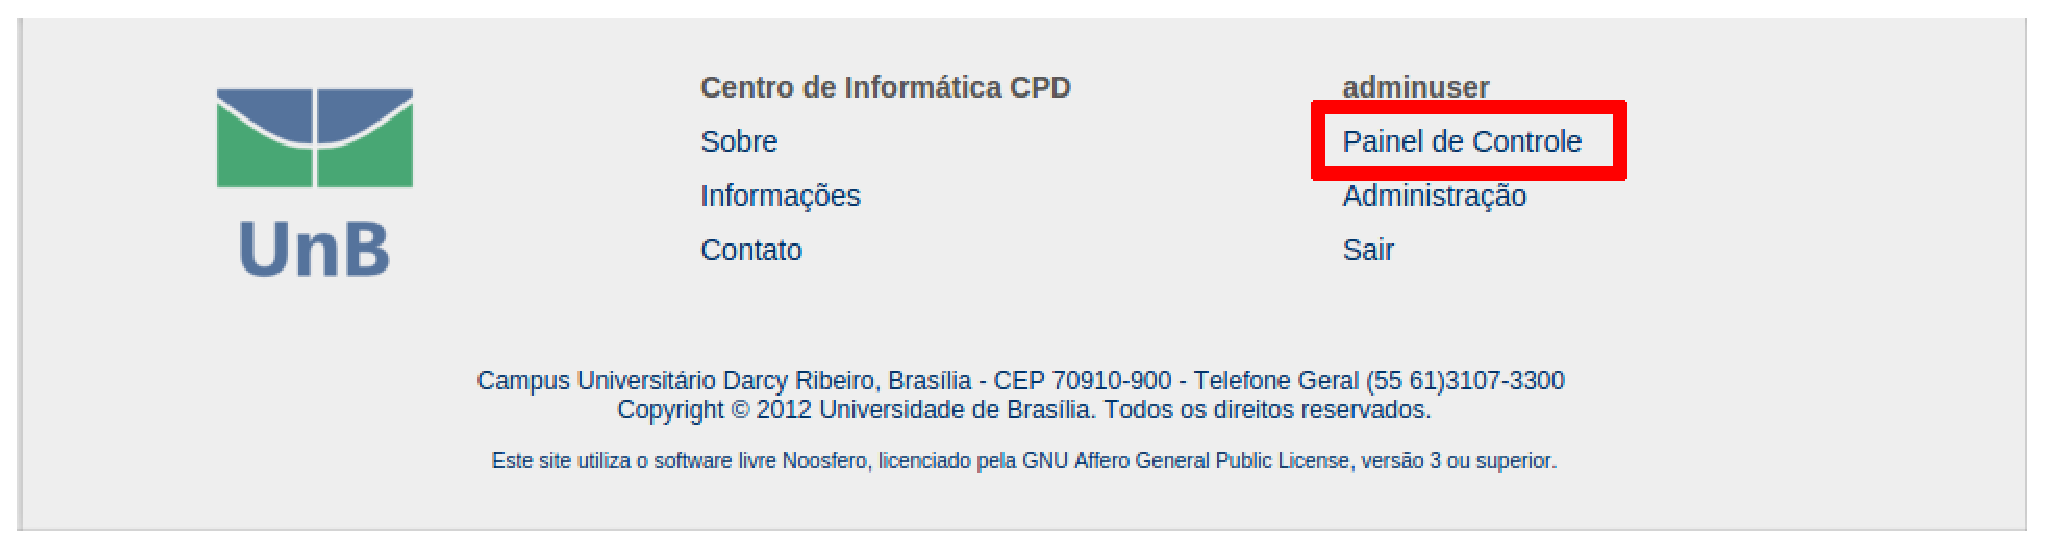
\includegraphics[keepaspectratio=true,scale=0.49]{figuras/linkPainelControle.eps} 
  \caption{Link para o Painel de Controle.}
  \label{fig:linkPainelControle}
\end{figure}

\newpage
Dentro do painel de controle, clique em \emph{\color{red}Gerenciar meus grupos}.

\begin{figure}[H]
  \centering
    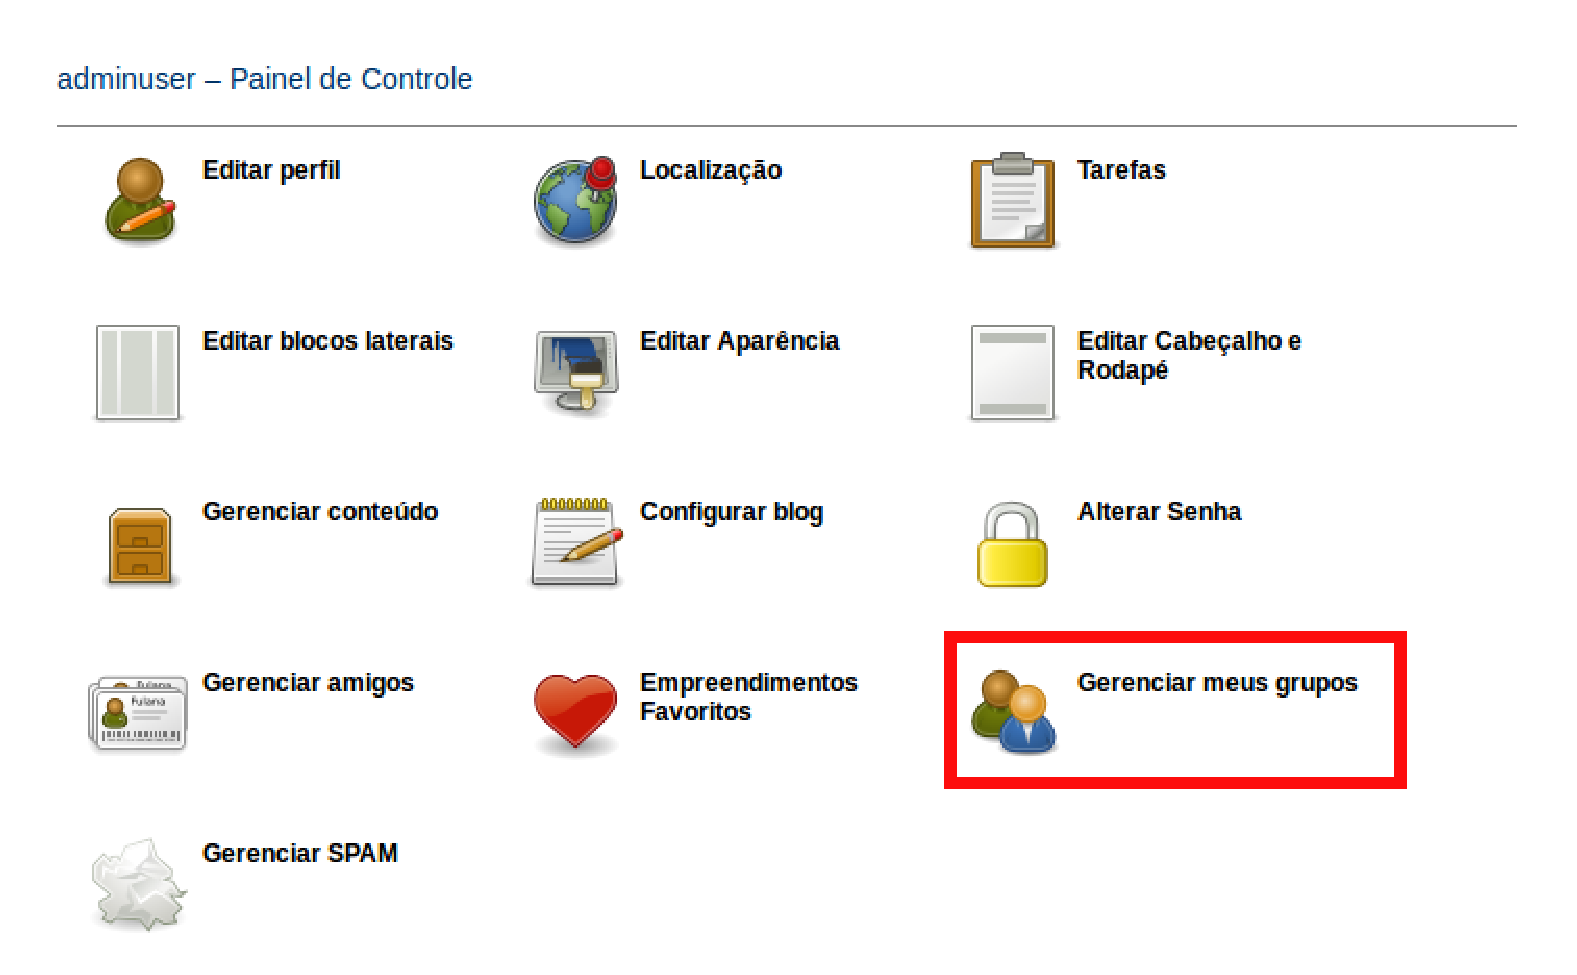
\includegraphics[keepaspectratio=true,scale=0.49]{figuras/painelDeControle.eps}
  \caption{Gerenciar grupos no painel de controle.}
  \label{fig:GerGrupPainelControle}
\end{figure}

Clique em \emph{\color{red}Painel de controle deste grupo} da comunidade na qual deseje criar o conteúdo.

\begin{figure}[H]
  \centering
    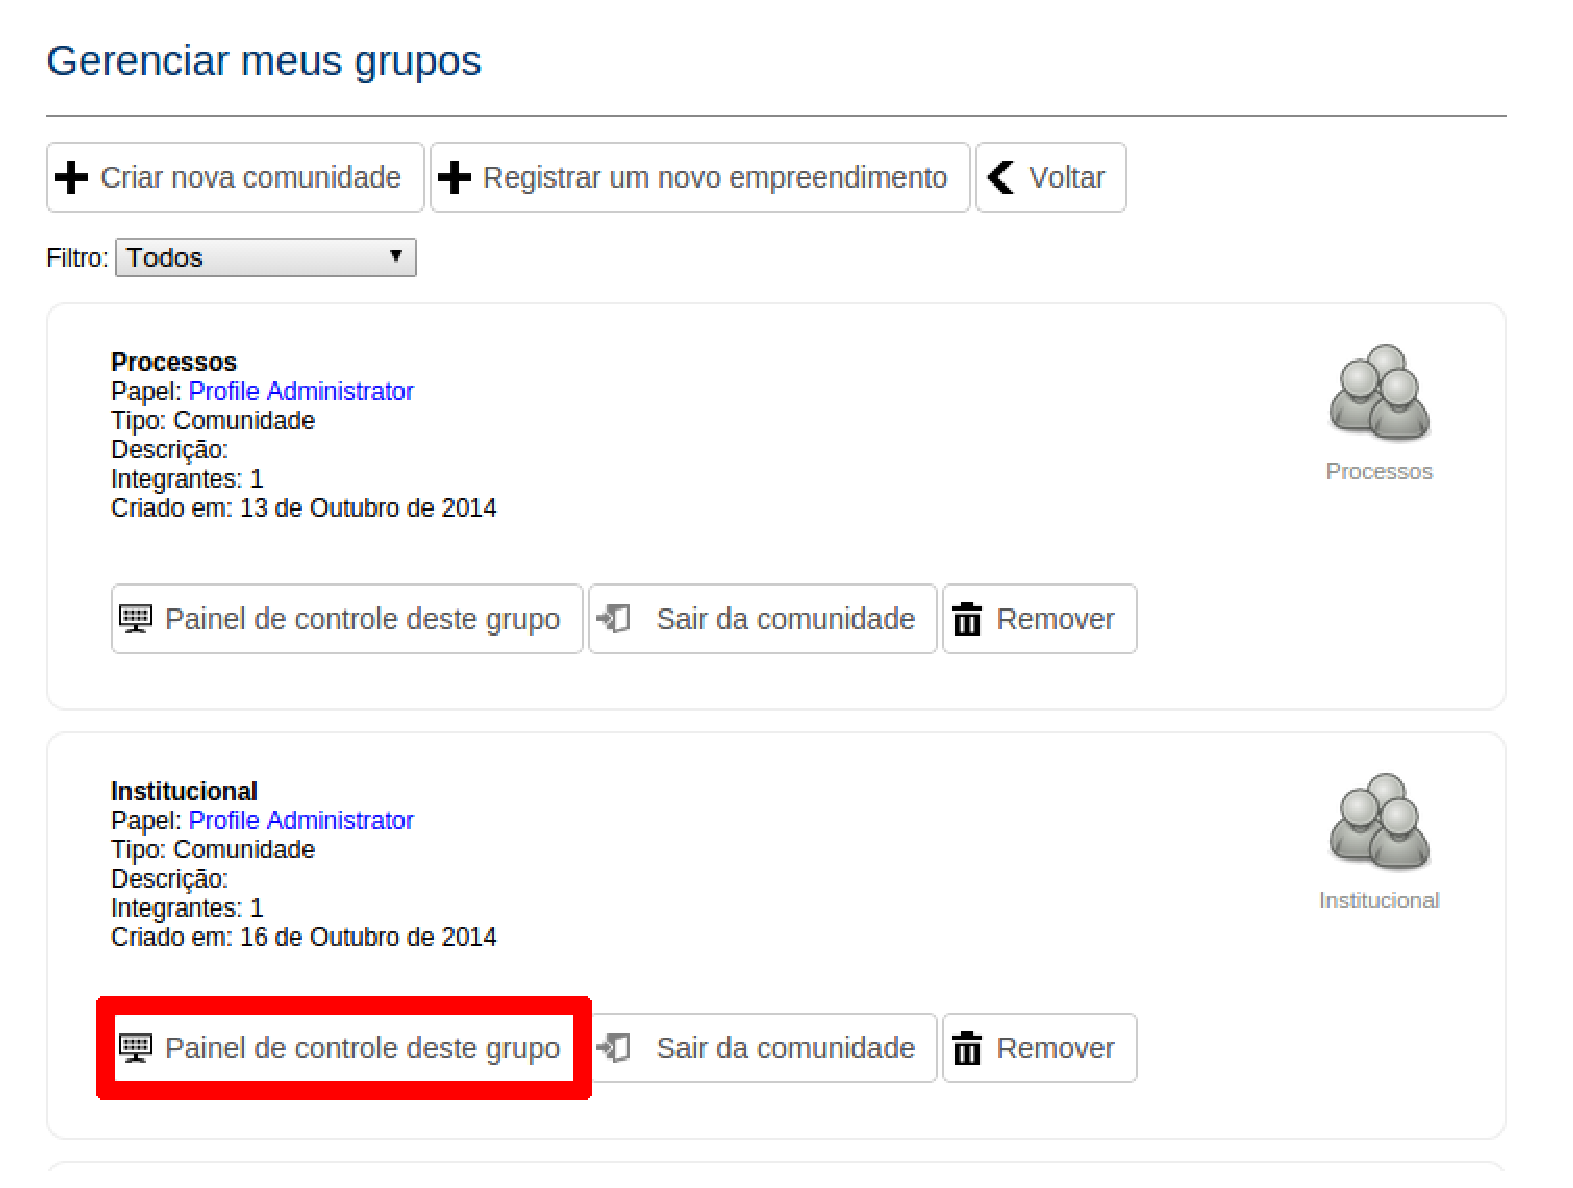
\includegraphics[keepaspectratio=true,scale=0.49]{figuras/selecionandoComunidade.eps}
  \caption{Entrar no Painel de Controle da Comunidade.}
  \label{fig:selecionandoComunidade}
\end{figure}

\newpage
Você será redirecionado para o Painel de Controle da comunidade selecionada, clique em \emph{\color{red}Gerenciar Conteúdo}.

\begin{figure}[H]
  \centering
    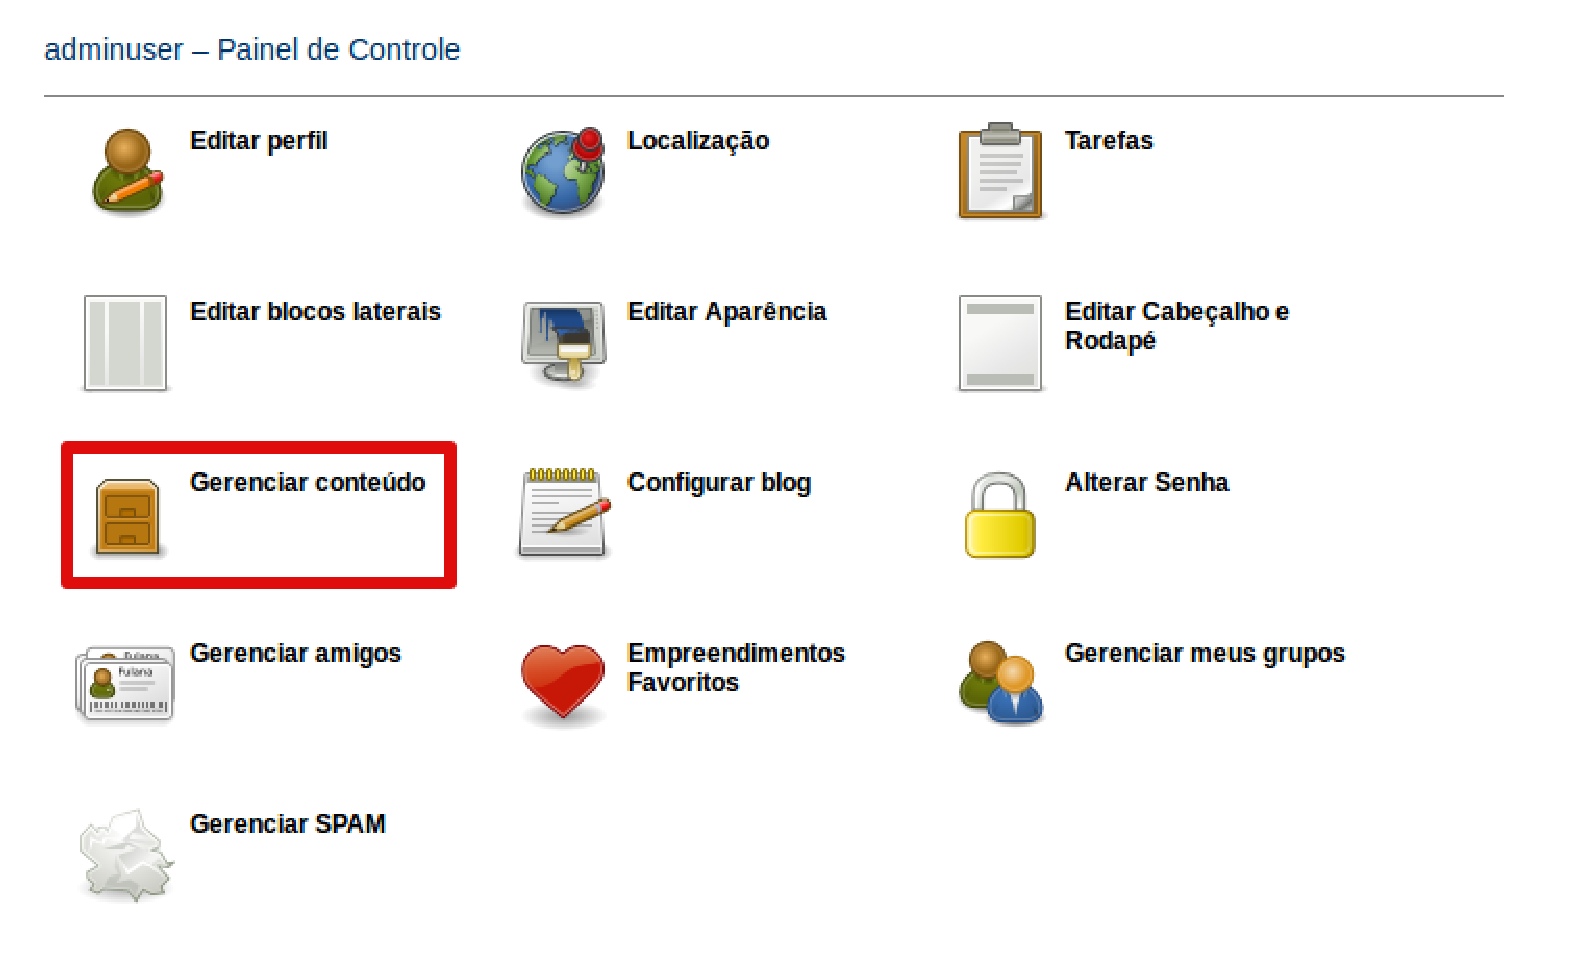
\includegraphics[keepaspectratio=true,scale=0.49]{figuras/painelControleGerenciarConteudo.eps}
  \caption{Painel de controle da comunidade.}
  \label{fig:GerContPainelControle}
\end{figure}

Agora clique em \emph{\color{red}Novo conteúdo}.

\begin{figure}[H]
  \centering
    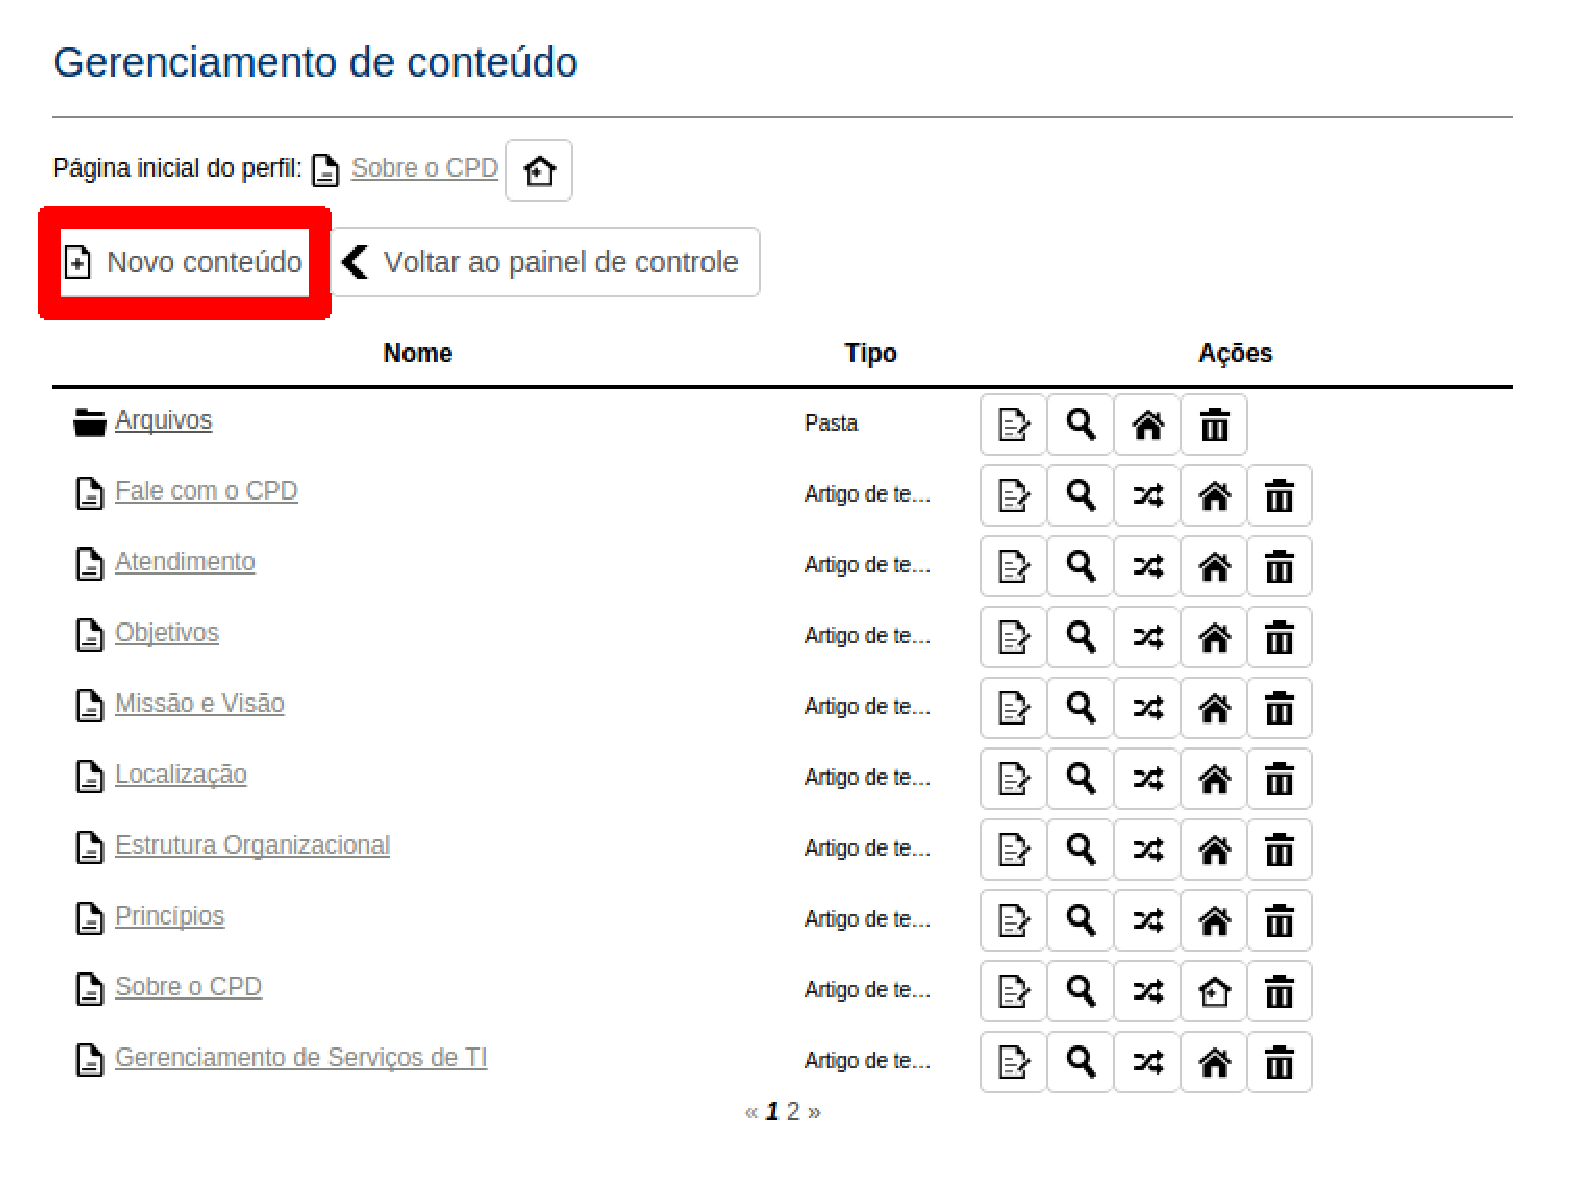
\includegraphics[keepaspectratio=true,scale=0.49]{figuras/novoConteudo.eps}
  \caption{Gerenciador de conteúdo da comunidade.}
  \label{fig:novoConteudo}
\end{figure}

Abrirá um janela, onde deve-se selecionar o tipo de conteúdo que se deseja criar. 

\subsection{Artigo}
\label{subsec:artigo}

Caso, queria criar um novo artigo, deve-se clicar em \emph{\color{red}Artigo de texto com editor visual}. Também pode-se optar por criar um \emph{\color{pink}Artigo de texto com HTML puro} caso deseje inserir conteúdo avançado em HTML puro.

\begin{figure}[H]
  \centering
    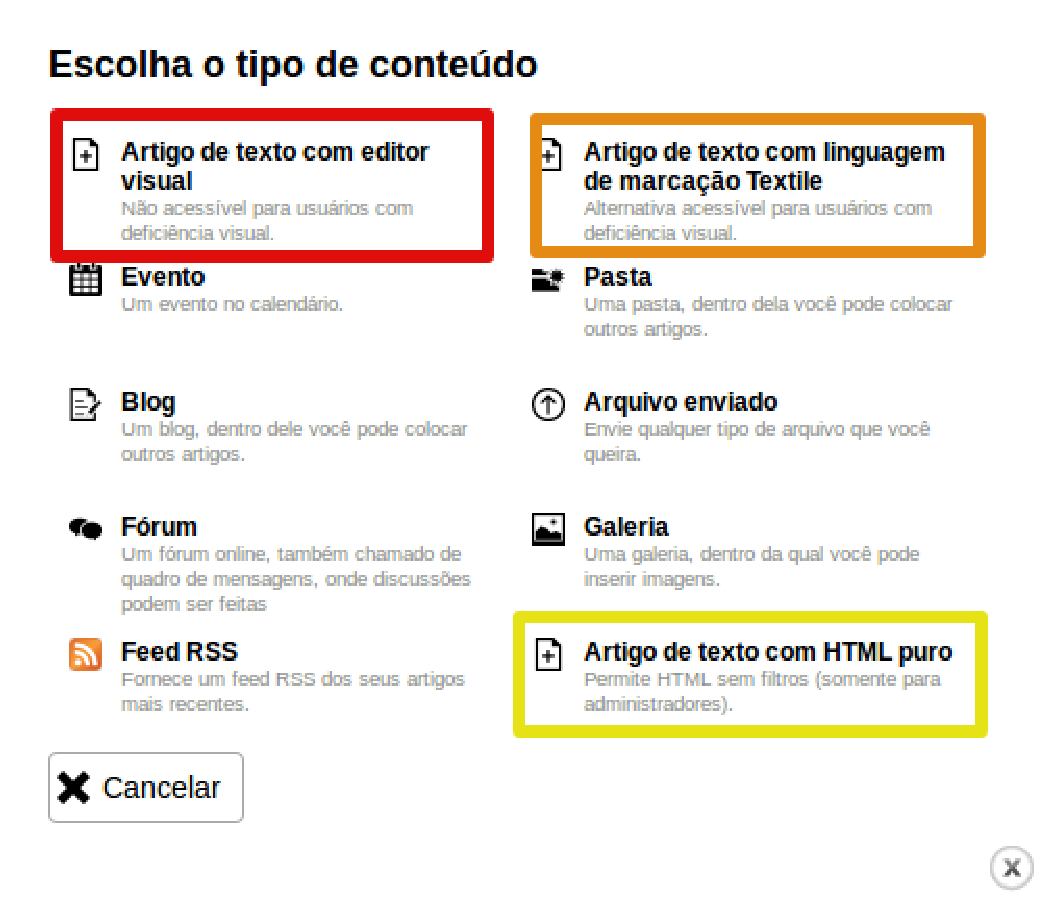
\includegraphics[keepaspectratio=true,scale=0.49]{figuras/criandoArtigo.eps}
  \caption{Escolha de conteúdo para criação: artigo.}
  \label{fig:FormCriacaoPasta}
\end{figure}

\subsection{Pasta}
\label{subsec:pasta}

A criação de pastas serve para melhor organização e categorização de conteúdos. Dentro de uma pasta, qualquer tipo de conteúdo suportado pelo Noosfero pode ser criado, incluindo artigos.

Se desejar criar uma pasta, clique em \emph{\color{red}Pasta}.

\begin{figure}[H]
  \centering
    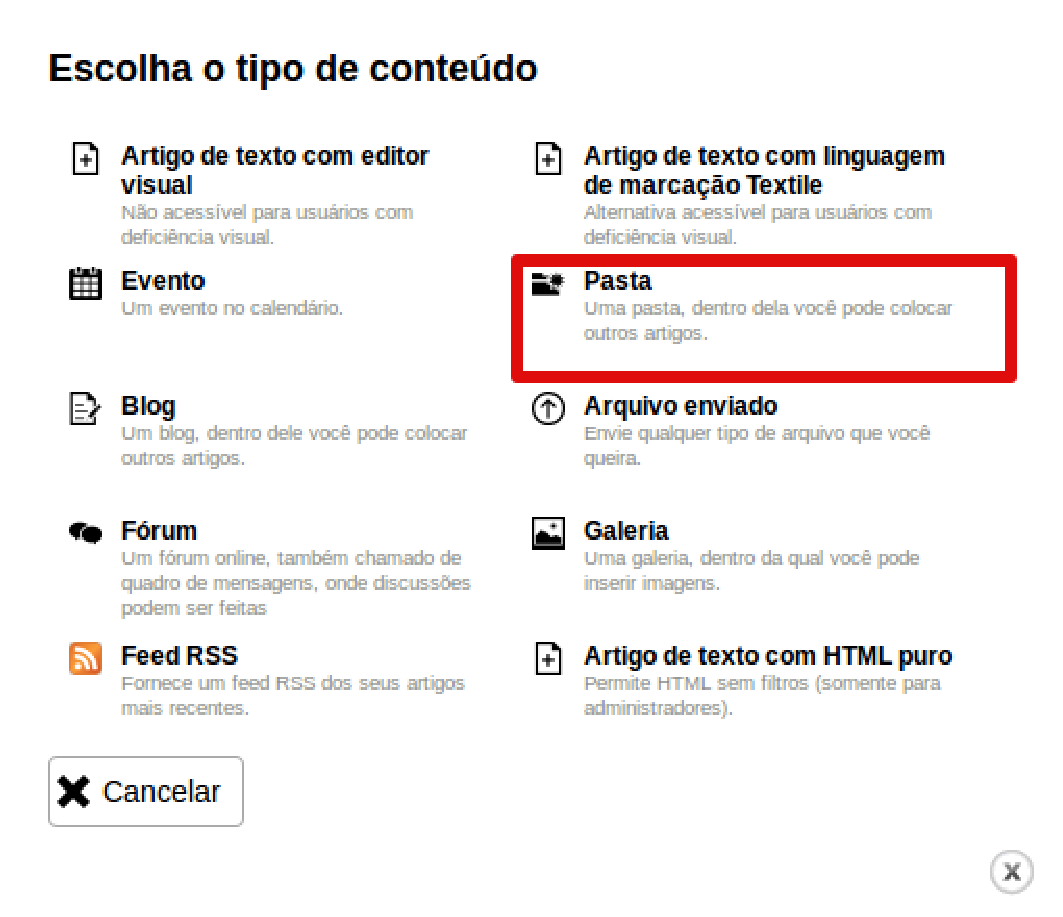
\includegraphics[keepaspectratio=true,scale=0.49]{figuras/escolhaConteudo.eps}
  \caption{Escolha de conteúdo para criação: pasta}
  \label{fig:GerenciamentoConteudo}
\end{figure}

Dê um nome à pasta em \emph{\color{red}Título}, e se desejar, insira uma descrição para a pasta no campo \emph{\color{pink}Descrição}. Para finalizar, clique em \emph{\color{red}Salvar}.

\begin{figure}[H]
  \centering
    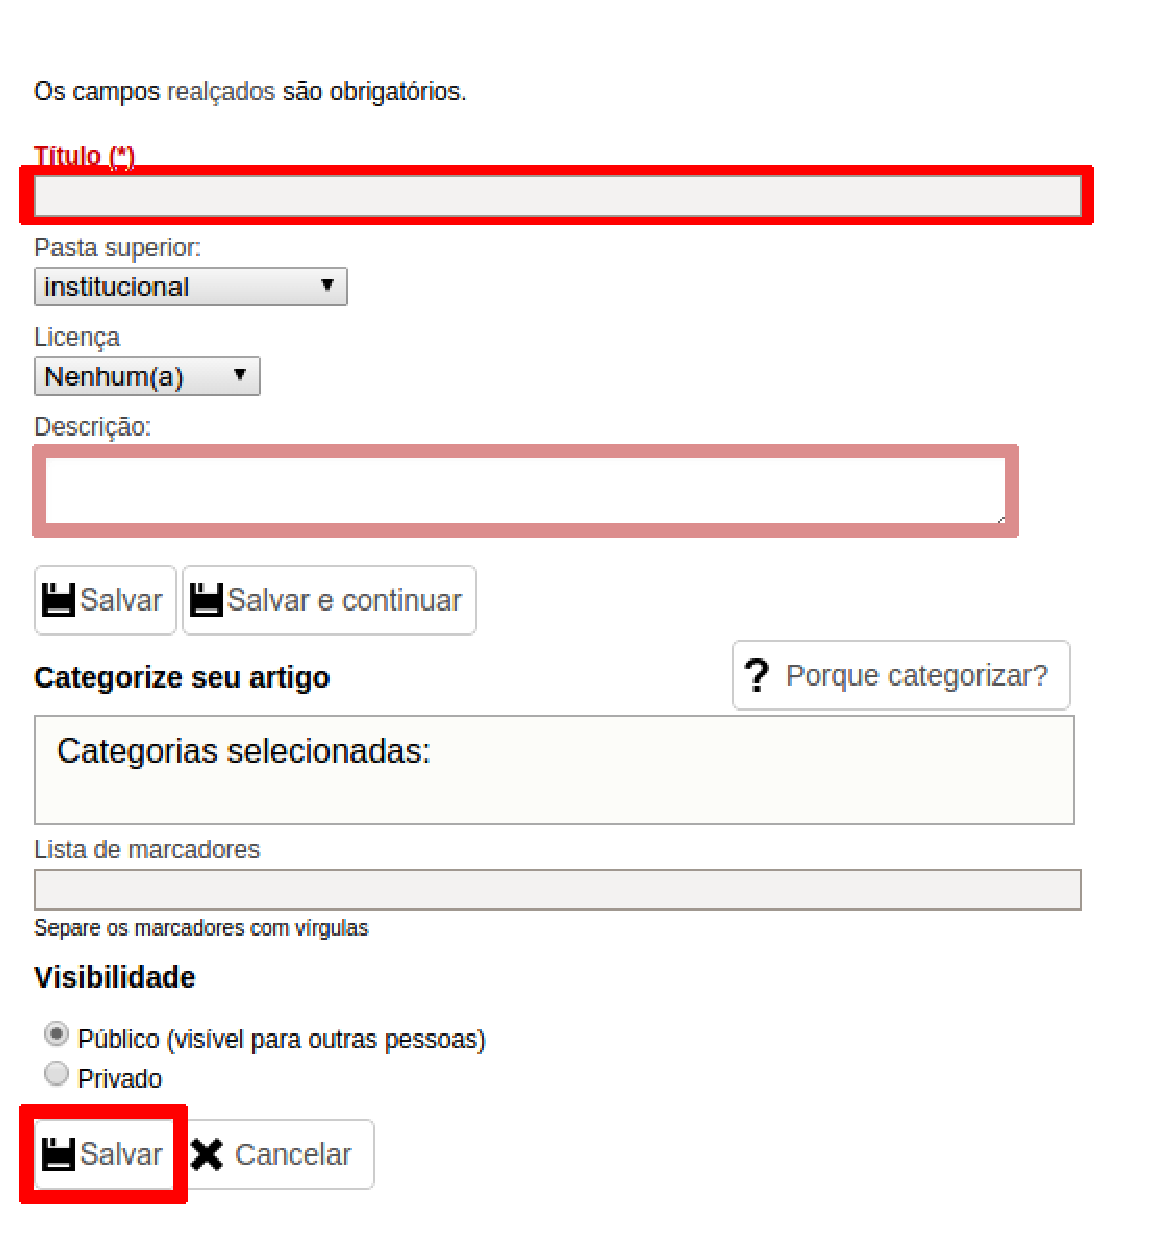
\includegraphics[keepaspectratio=true,scale=0.49]{figuras/criandoPasta.eps}
  \caption{Formulário de criação de pasta.}
  \label{fig:FormCriacaoPasta}
\end{figure}

\subsection{Blog}
\label{subsec:blog}

No Noosfero também é possível a criação de blogs, sendo que numa comunidade podem existir quantos blogs o usuário desejar.

Clique em \emph{\color{red}Blog} para cria um novo blog.

\begin{figure}[H]
  \centering
    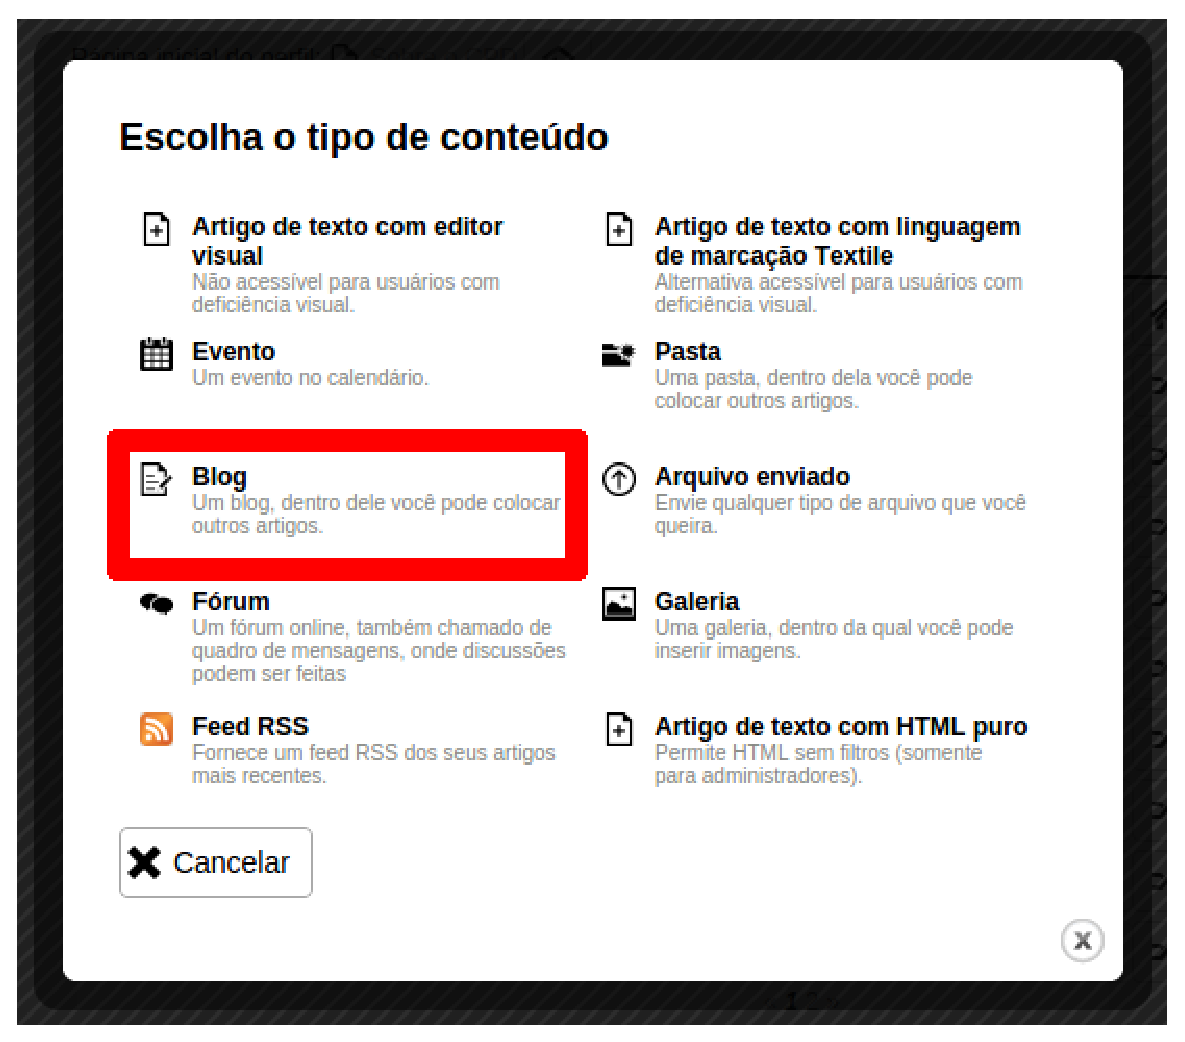
\includegraphics[keepaspectratio=true,scale=0.49]{figuras/selecionarBlog.eps}
  \caption{Escolha de conteúdo para criação: blog}
  \label{fig:selecionarBlog}
\end{figure}

\newpage
Dê um nome ao blog em \emph{Título}, se desejar insira uma descrição para a pasta no campo \emph{Descrição}. Defina se deseja se o blog exiba os artigos completos, ou se apenas um resumo em \emph{Mostrar posts como}, e quantos artigos devem ser exibidos por página em \emph{Posts por página} e finalmente clique em \emph{\color{red}Salvar}.

\begin{figure}[H]
  \centering
    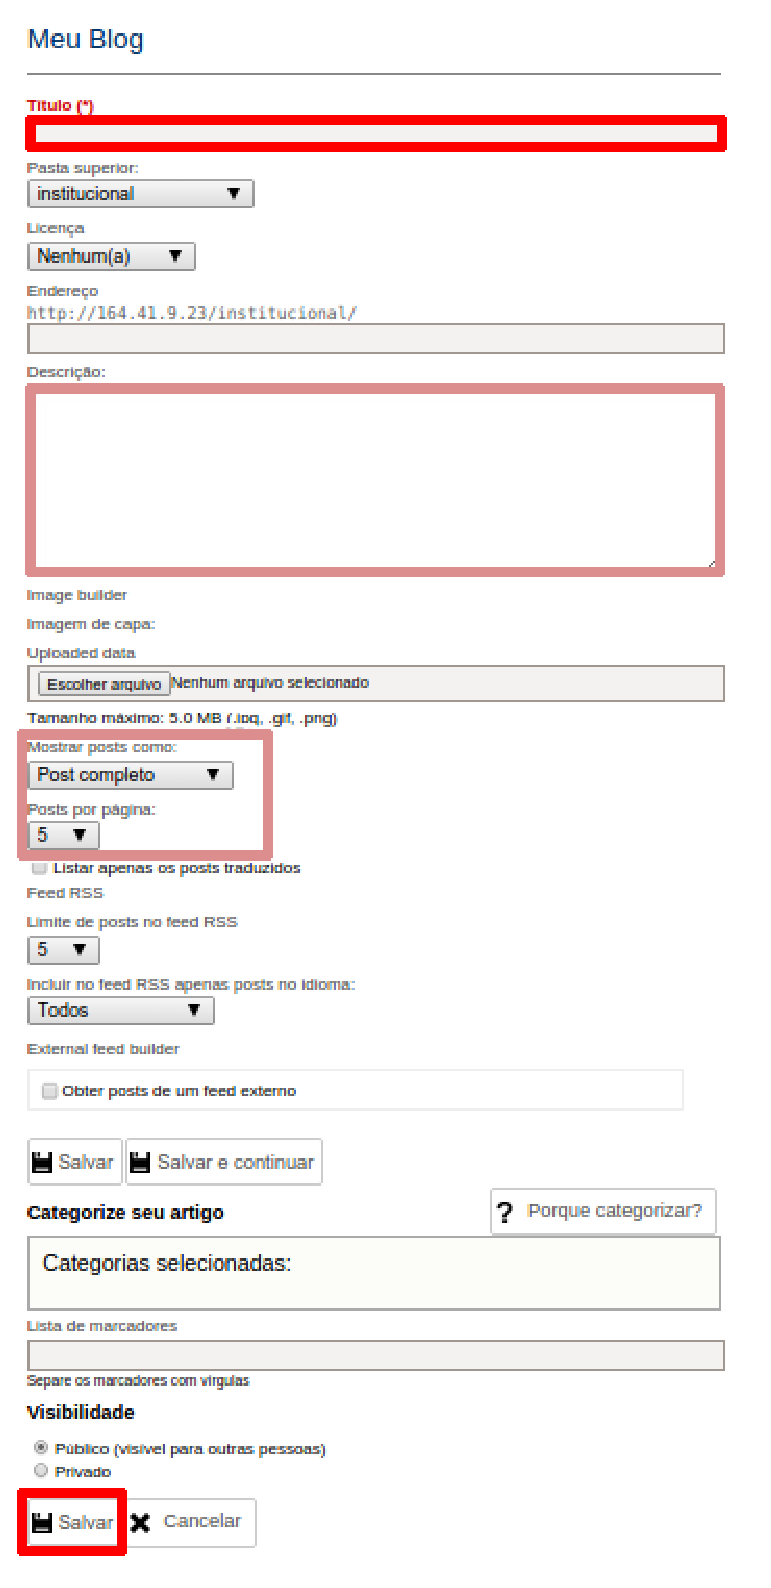
\includegraphics[keepaspectratio=true,scale=0.49]{figuras/criandoBlog.eps}
  \caption{Formulário de criação do blog.}
  \label{fig:FormCriacaoBlog}
\end{figure}

